% Intended LaTeX compiler: xelatex
\documentclass[10pt, svgnames]{beamer}
\usepackage{graphicx}
\usepackage{longtable}
\usepackage{wrapfig}
\usepackage{rotating}
\usepackage[normalem]{ulem}
\usepackage{amsmath}
\usepackage{amssymb}
\usepackage{capt-of}
\usepackage{hyperref}
\usetheme{metropolis}
\author{Sappinandana Akamphon}
\date{\today}
\title{Introduction to Engineering Design}
\subtitle{ME 310: Mechanical Design}
\usepackage{booktabs}
\usepackage{pgfplots}
\usepackage{multirow}
\usepackage{wasysym}
\usepackage{array}
\pgfplotsset{compat=1.18}
\institute{Department of Mechanical Engineering, TSE}
\usetikzlibrary{patterns,shapes,arrows,decorations,decorations.pathmorphing,calc}
\AtBeginSection[]{\begin{frame}{Outline}\tableofcontents[currentsection]\end{frame}}
\definecolor{lightblue}{RGB}{180,220,255}
\tikzset{/pgf/decoration/.cd,
head width/.initial=6pt,
head length/.initial=1.5pt,
thread separation/.initial=1.0pt,
thread amplitude/.initial=.meta0.5pt,
screw radius/.initial=1.2pt,}
% definition of the decoration
\pgfdeclaredecoration{screw}{initial}
{
\state{initial}[width=\pgfkeysvalueof{/pgf/decoration/head length},%
next state=midd]
{
\def\headlength{%
\pgfkeysvalueof{/pgf/decoration/head length}%
}
\def\headwidth{%
\pgfkeysvalueof{/pgf/decoration/head width}%
}
\def\screwradius{%
\pgfkeysvalueof{/pgf/decoration/screw radius}%
}
% First line
\pgfpathlineto{\pgfpoint{0.0pt}{\headwidth/2}}
\pgfpathlineto{\pgfpoint{\headlength}{\headwidth/2}}
\pgfpathlineto{\pgfpoint{\headlength}{\screwradius}}
% Second line
\pgfpathmoveto{\pgfpoint{0.0pt}{0.0pt}}
\pgfpathlineto{\pgfpoint{0.0pt}{-\headwidth/2}}
\pgfpathlineto{\pgfpoint{\headlength}{-\headwidth/2}}
\pgfpathlineto{\pgfpoint{\headlength}{-\screwradius}}
}
\state{midd}[width=\pgfkeysvalueof{/pgf/decoration/thread separation}*2]
{
\def\threadseparation{%
\pgfkeysvalueof{/pgf/decoration/thread separation}%
}
\def\threadamplitude{%
\pgfkeysvalueof{/pgf/decoration/thread amplitude}%
}
\def\screwradius{%
\pgfkeysvalueof{/pgf/decoration/screw radius}%
}
% First line
\pgfpathmoveto{\pgfpoint{0pt}{\screwradius}}
\pgfpathlineto{\pgfpoint{0.5*\threadseparation}{\screwradius+\threadamplitude}}
\pgfpathlineto{\pgfpoint{1.0*\threadseparation}{\screwradius}}
\pgfpathlineto{\pgfpoint{1.5*\threadseparation}{\screwradius-\threadamplitude}}
\pgfpathlineto{\pgfpoint{2.0*\threadseparation}{\screwradius}}
% Second line
\pgfpathmoveto{\pgfpoint{0pt}{-\screwradius}}
\pgfpathlineto{\pgfpoint{0.5*\threadseparation}{-\screwradius-\threadamplitude}}
\pgfpathlineto{\pgfpoint{1.0*\threadseparation}{-\screwradius}}
\pgfpathlineto{\pgfpoint{1.5*\threadseparation}{-\screwradius+\threadamplitude}}
\pgfpathlineto{\pgfpoint{2.0*\threadseparation}{-\screwradius}}
% Thread
\pgfpathmoveto{\pgfpoint{0.5*\threadseparation}{\screwradius+\threadamplitude}}
\pgfpathlineto{\pgfpoint{1.5*\threadseparation}{-\screwradius+\threadamplitude}}
}
\state{final}
{
\def\screwradius{%
\pgfkeysvalueof{/pgf/decoration/screw radius}%
}
%\pgfpathlineto{\pgfpointdecoratedpathlast}
\pgfpathmoveto{\pgfpoint{0pt}{\screwradius}}
\pgfpathlineto{\pgfpoint{\screwradius/2}{0pt}}
\pgfpathlineto{\pgfpoint{0pt}{-\screwradius}}
}
}
\hypersetup{
 pdfauthor={Sappinandana Akamphon},
 pdftitle={Introduction to Engineering Design},
 pdfkeywords={},
 pdfsubject={},
 pdfcreator={Emacs 30.0.50 (Org mode 9.6)}, 
 pdflang={English}}
\begin{document}

\maketitle

\section{Overview of Bolted Joints}
\label{sec:org3f98797}

\begin{frame}[label={sec:org96846f8}]{Bolted Joints}
Bolted joints are held by threaded fasteners
\begin{itemize}
\item Bolts
\item Screws
\item Nuts
\end{itemize}

What's the difference between a bolt and a screw?
\end{frame}

\begin{frame}[label={sec:org92b9db6}]{How Bolted Joints Work}
\begin{itemize}
\item Clamped members are held together by compressive load from a bolt or screw
\item Bolt itself is under tensile load
\end{itemize}
\end{frame}

\begin{frame}[label={sec:org4e2513b}]{Applications of Bolted Joints}
\begin{figure}[h]
  \centering
  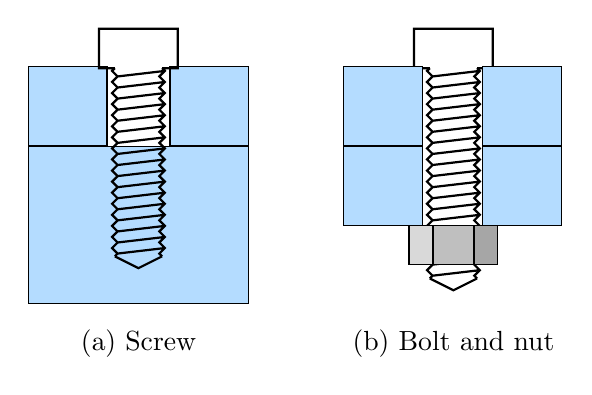
\begin{tikzpicture}
    % clamped members
    \node at (0,-0.5) [anchor=south,draw, rectangle, fill=lightblue, minimum width=2.8cm, minimum height=2cm](A){};
    \node at (A.north west) [anchor=south west,draw, rectangle, fill=lightblue, minimum width=1cm, minimum height=1cm]{};
    \node at (A.north east) [anchor=south east,draw, rectangle, fill=lightblue, minimum width=1cm, minimum height=1cm]{};
    % bolt
    \draw[decorate,thick,decoration={screw, screw radius=0.3cm, thread amplitude=1pt, thread separation=2pt, head width=1.0cm, head length=0.5cm}] (0,3) -- (0,0);
    % description
    \node at (0,-1) {(a) Screw};
     % bolt
    \draw[decorate,thick,decoration={screw, screw radius=0.3cm, thread amplitude=1pt, thread separation=2pt, head width=1.0cm, head length=0.5cm}] (4,3) -- (4,-0.25);
    % clamped members
    \node at (2.6,0.5) [anchor=south west,draw, rectangle, fill=lightblue, minimum width=1cm, minimum height=1cm](A){};
    \node at (A.south east) [anchor=south west,draw, rectangle, fill=lightblue, minimum width=1cm, minimum height=1cm, xshift=0.75cm](B){};
    \node at (A.north) [anchor=south,draw, rectangle, fill=lightblue, minimum width=1cm, minimum height=1cm]{};
    \node at (B.north) [anchor=south,draw, rectangle, fill=lightblue, minimum width=1cm, minimum height=1cm]{};
    % nut
    \node at (4,0) [anchor=south, draw, rectangle, fill=Grey!50, minimum height=0.5cm, minimum width=0.5cm](C){};
    \node at (C.east) [anchor=west, draw, rectangle, fill=Grey!70, minimum height=0.5cm, minimum width=0.3cm]{};
    \node at (C.west) [anchor=east, draw, rectangle, fill=Grey!30, minimum height=0.5cm, minimum width=0.3cm]{};
    % description
    \node at (4,-1) {(b) Bolt and nut};
  \end{tikzpicture}
\end{figure}
\end{frame}

\begin{frame}[label={sec:org02206da}]{Application of Bolted Joints 2}
\begin{figure}[h]
  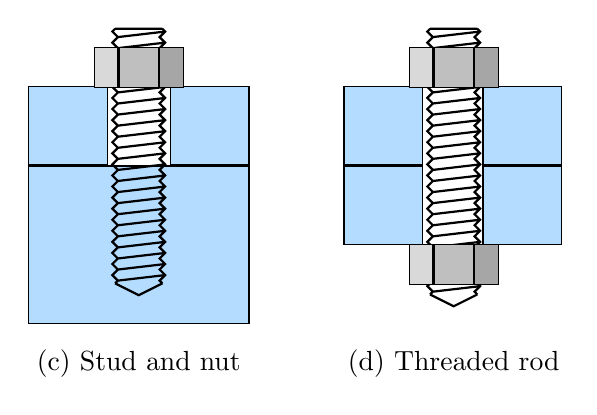
\begin{tikzpicture}
    % clamped members
    \node at (8,-0.5) [anchor=south,draw, rectangle, fill=lightblue, minimum width=2.8cm, minimum height=2cm](D){};
    \node at (D.north west) [anchor=south west,draw, rectangle, fill=lightblue, minimum width=1cm, minimum height=1cm]{};
    \node at (D.north east) [anchor=south east,draw, rectangle, fill=lightblue, minimum width=1cm, minimum height=1cm]{};
    % bolt
    \draw[decorate,thick,decoration={screw, screw radius=0.3cm, thread amplitude=1pt, thread separation=2pt, head width=0cm, head length=0cm}] (8,3.25) -- (8,0);
    % nut
    \node at (8,2.5) [anchor=south, draw, rectangle, fill=Grey!50, minimum height=0.5cm, minimum width=0.5cm](E){};
    \node at (E.east) [anchor=west, draw, rectangle, fill=Grey!70, minimum height=0.5cm, minimum width=0.3cm]{};
    \node at (E.west) [anchor=east, draw, rectangle, fill=Grey!30, minimum height=0.5cm, minimum width=0.3cm]{};
    % description
    \node at (8,-1) {(c) Stud and nut};
   % bolt
    \draw[decorate,thick,decoration={screw, screw radius=0.3cm, thread amplitude=1pt, thread separation=2pt, head width=0cm, head length=0cm}] (12,3.25) -- (12,-0.25);
    % clamped members
    \node at (10.6,0.5) [anchor=south west,draw, rectangle, fill=lightblue, minimum width=1cm, minimum height=1cm](F){};
    \node at (F.south east) [anchor=south west,draw, rectangle, fill=lightblue, minimum width=1cm, minimum height=1cm, xshift=0.75cm](G){};
    \node at (F.north) [anchor=south,draw, rectangle, fill=lightblue, minimum width=1cm, minimum height=1cm]{};
    \node at (G.north) [anchor=south,draw, rectangle, fill=lightblue, minimum width=1cm, minimum height=1cm]{};
    % bottom nut
    \node at (12,0) [anchor=south, draw, rectangle, fill=Grey!50, minimum height=0.5cm, minimum width=0.5cm](H){};
    \node at (H.east) [anchor=west, draw, rectangle, fill=Grey!70, minimum height=0.5cm, minimum width=0.3cm]{};
    \node at (H.west) [anchor=east, draw, rectangle, fill=Grey!30, minimum height=0.5cm, minimum width=0.3cm]{};
  % top nut
    \node at (12,2.5) [anchor=south, draw, rectangle, fill=Grey!50, minimum height=0.5cm, minimum width=0.5cm](I){};
    \node at (I.east) [anchor=west, draw, rectangle, fill=Grey!70, minimum height=0.5cm, minimum width=0.3cm]{};
    \node at (I.west) [anchor=east, draw, rectangle, fill=Grey!30, minimum height=0.5cm, minimum width=0.3cm]{};
  % description
    \node at (12,-1) {(d) Threaded rod};
  \end{tikzpicture}
\end{figure}
\end{frame}

\section{Bolt Geometry and Properties}
\label{sec:org3de434d}

\begin{frame}[label={sec:org8395a0a}]{Thread Geometry}
\centering
\includegraphics[width=\textwidth]{pictures/screw-thread-forms}
\end{frame}

\begin{frame}[label={sec:orgdc92b23}]{Thread Forms}
\begin{figure}[h]
  \centering
  \includegraphics[scale=1]{pictures/bolt-terminology}
\end{figure}
\end{frame}

\begin{frame}[label={sec:org9862867}]{Standard ISO Bolt Sizes}
\scriptsize
\begin{tabular}{ p{1.2cm} p{1cm} p{1cm} p{1.3cm} p{1cm} p{1cm} p{1.3cm}}
  \toprule
  \multirow{2}{1.5cm}{Nominal Diameter $d$} & \multicolumn{3}{c}{Coarse Threads} & \multicolumn{3}{c}{Fine Threads} \\ \cmidrule{2-7}
                                            & Pitch & Minor $\diameter$ & Stress Area & Pitch & Minor $\diameter$ & Stress Area \\
  \midrule
  3   & 0.5  & 2.39 & 5.03 & -    & -    & - \\
  3.5 & 0.6  & 2.76 & 6.78 & -    & -    & - \\
  4   & 0.7  & 3.14 & 8.78 & -    & -    & - \\
  5   & 0.8  & 4.02 & 14.2 & -    & -    & - \\
  6   & 1    & 4.77 & 20.1 & -    & -    & - \\
  7   & 1    & 5.77 & 28.9 & -    & -    & - \\
  8   & 1.25 & 6.47 & 36.6 & 1    & 6.77 & 39.2 \\
  10  & 1.5  & 8.16 & 58.0 & 1.25 & 8.47 & 61.2 \\
  12  & 1.75 & 9.85 & 84.3 & 1.25 & 10.5 & 92.1 \\
  14  & 2    & 11.6 & 115  & 1.5  & 12.2 & 125 \\
  16  & 2    & 13.6 & 157  & 1.5  & 14.2 & 167 \\
  18  & 2.5  & 14.9 & 192  & 1.5  & 16.2 & 216 \\
  20  & 2.5  & 16.9 & 245  & 1.5  & 18.2 & 272 \\
  22  & 2.5  & 18.9 & 303  & 1.5  & 20.2 & 333 \\
  24  & 3    & 20.3 & 353  & 2    & 21.6 & 384 \\
  27  & 3    & 23.3 & 459  & 2    & 24.6 & 496 \\
  30  & 3.5  & 25.7 & 561  & 2    & 27.6 & 621 \\
  33  & 3.5  & 28.7 & 694  & 2    & 30.6 & 761 \\
  36  & 4    & 31.1 & 817  & 3    & 32.3 & 865 \\
  39  & 4    & 34.1 & 976  & 3    & 35.3 & 1030 \\
  42  & 4.5  & 36.9 & 1121 & -    & -    & - \\
  48  & 5    & 42.7 & 1473 & -    & -    & - \\
  \bottomrule
\end{tabular}
\end{frame}

\begin{frame}[label={sec:orgd6510ad}]{How are Screw Threads Made?: Thread Rolling}
\begin{figure}[h]
  \centering
  \includegraphics[width=0.9\textwidth]{pictures/thread-rolling}
\end{figure}
\end{frame}

\begin{frame}[label={sec:org0ea12ec}]{How are Screw Threads Made?: Thread Cutting}
\begin{figure}[h]
  \centering
  \includegraphics[width=0.7\textwidth]{pictures/thread-cutting}
\end{figure}
\end{frame}

\begin{frame}[label={sec:org57b5fdf}]{Advantage of Rolled vs Cut Threads}
\begin{figure}[h]
  \centering
  \includegraphics[width=0.9\textwidth]{pictures/cut-rolled-thread}
\end{figure}
\end{frame}

\begin{frame}[label={sec:orgb4d0726}]{Strength of Bolts}
\begin{itemize}
\item Because of threads and how they are formed, bolts are not loaded to their yield or ultimate tensile strength.
\item Instead, bolt strength is measured by a \emph{proof strength}, $S_p$.
\item For approximation, $S_p = 0.9 S_y$
\end{itemize}
\end{frame}

\begin{frame}[label={sec:orga94c203}]{Bolt Material Strength}
\small
\begin{tabular}{ p{0.8cm} p{1.2cm} p{1.2cm} p{1.2cm} p{1.5cm} p{1.5cm} p{1.3cm} }
  \toprule
  SAE Class & Diameter $d$ (mm) & Proof Strength $S_p$ (MPa) & Yield Strength $S_y$ (MPa) & Tensile Strength $S_{ut}$ (MPa) & Elongation (\%) & Reduction of Area (\%) \\
  \midrule
  4.6 & 5 – 36 & 225 & 240 & 400 & 22 & 35 \\
  4.8 & 1.6 – 16 & 310 & - & 420 & - & - \\
  5.8 & 5 – 24 & 380 & - & 520 & - & - \\
  8.8 & 17 – 36 & 600 & 660 & 830 & 12 & 12 \\
  9.8 & 1.6 – 16 & 650 & - & 900 & - & - \\
  10.9 & 6 – 36 & 830 & 940 & 1040 & 9 & 9 \\
  12.9 & 1.6 – 36 & 970 & 1100 & 1220 & 8 & 8 \\
  \bottomrule
\end{tabular}
\end{frame}

\begin{frame}[label={sec:org4cc3183}]{Head Markings Example}
\begin{figure}[h]
  \centering
  \includegraphics[width=0.9\textwidth]{pictures/metric-head-markings}
\end{figure}
\end{frame}

\section{Bolt Stress Analysis}
\label{sec:orgb3a9244}

\begin{frame}[label={sec:orgb62d8b5}]{Bolted Joint Stress Analysis}
\begin{itemize}
  \item Two modes of failure
  \item Thread failure $\rightarrow$ shear stress in thread
  \item Tensile faiure $\rightarrow$ tensile stress in bolt
\end{itemize}
\end{frame}

\begin{frame}[label={sec:org3982c6f}]{Shear Stress in Threads}
\begin{columns}
  \begin{column}{0.5\textwidth}
    \begin{itemize}
      \item Thread surface area is
            $$ A_{shear} = \pi d (0.75 t) $$
      \item Allowable shear stress on bolt (MDET)
            \begin{equation*}
              \tau_{allow} = \frac{S_{y}}{\sqrt{3}} = 0.577S_{y}
            \end{equation*}
      \item Force to cause thread failure
            \begin{equation*}
              F_{thread} = 0.577S_{y}\pi d (0.75) t
            \end{equation*}
    \end{itemize}
  \end{column}
  \begin{column}{0.5\textwidth}
        \begin{figure}[h]
          \centering
          \includegraphics[scale=0.6]{pictures/bolt-terminology}
        \end{figure}
  \end{column}
\end{columns}
\end{frame}

\begin{frame}[label={sec:org94c8ffa}]{Bolt Tensile Stress}
\begin{itemize}
  \item Bolt tensile area
        \begin{equation*}
          A_{t} \approx \frac{\pi}{4}\left(0.9d\right)^{2}
        \end{equation*}
  \item Tensile load to yield the bolt threads
        \begin{equation*}
          F_{bolt} = A_t S_y \approx \frac{\pi}{4}(0.9d)^2 S_y
        \end{equation*}
\end{itemize}
\end{frame}

\begin{frame}[label={sec:orgf5ce50a}]{Preventing Thread Failure}
\begin{itemize}
  \item To prevent thread failure, make sure tensile failure happens first (or at the same time)
  \item Setting $F_{bolt} = F_{nut}$
  $$ t = 0.47d $$
  \item The thickness nut or depth of threaded hole should be at least half major diameter.
  \item Now we can worry only about tensile failure
\end{itemize}
\end{frame}

\begin{frame}[label={sec:orgf03309a}]{Torque - Tensile Load Relationship}
\begin{itemize}
\item Setting $\mu = 0.15$

  $$ T = 0.2{F_i}d $$

\item Metal on metal friction is 0.15?
\end{itemize}
\end{frame}

\begin{frame}[label={sec:orgb21d4cd}]{Proper Bolted Joints}
\begin{itemize}
\item Correct bolt length and proper nut/threaded hole thickness
  $$ t \geqslant 0.47d $$
\item Proper tightening with calculated torque $\rightarrow$ torque wrench is your friend
\item Locking mechanism: locknuts, slotted nuts, two nuts, toothed lock washers.
\end{itemize}
\begin{figure}[htbp]
  \centering
  \includegraphics[height=0.3\textheight]{pictures/locknut}
  \includegraphics[height=0.3\textheight]{pictures/lock-washer}
  \includegraphics[height=0.3\textheight]{pictures/slotted-nut}
\end{figure}
\end{frame}

\begin{frame}[label={sec:org6822844}]{Bolt-Joint Interaction}
\begin{figure}[h]
  \centering
  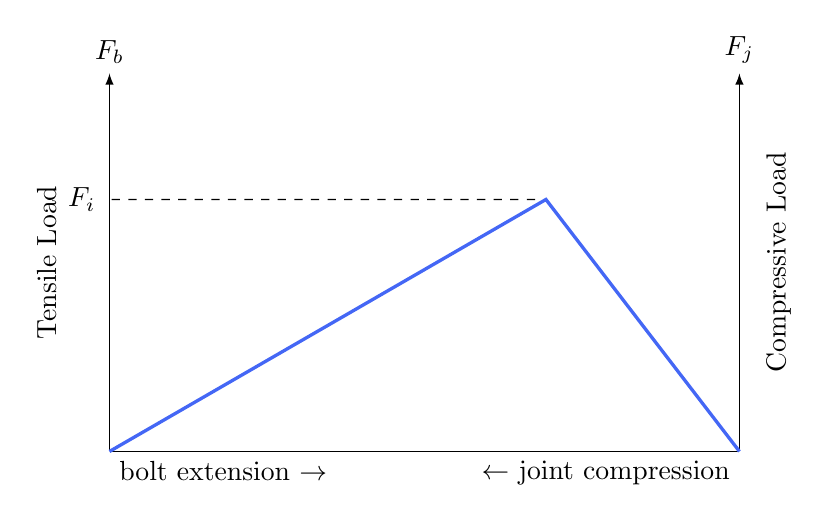
\begin{tikzpicture}[scale=0.8, >=latex]
    \draw [->] (0,0) node(A){} node[below right]{bolt extension $\rightarrow$} --++ (90:6) node[above]{$F_b$} node[midway, xshift=-8mm, rotate=90]{Tensile Load};
    \draw (0,0) --++ (0:10);
    \draw [->, xshift=10cm] (0,0) node(B){} node[below left]{$\leftarrow$ joint compression} --++ (90:6) node[above]{$F_j$} node[midway, xshift=5mm, rotate=90]{Compressive Load};
    \draw [SkyBlue!50!Blue, very thick](A.center) --++ (30:8) node(C){} -- (B.center);
    \draw [dashed] (C) -- ++ (180:7) node[left]{$F_i$};
  \end{tikzpicture}
\end{figure}
\end{frame}

\begin{frame}[label={sec:orgdfc6760}]{Types of Bolted Joints}
\begin{itemize}
\item Tension Joints
\item Friction Joints
\end{itemize}
\centering
\includegraphics[height=0.5\textheight]{pictures/joint-types}
\end{frame}

\begin{frame}[label={sec:org2707c26}]{Load Distribution in Tension Joints}
 \begin{figure}[h]
  \centering
  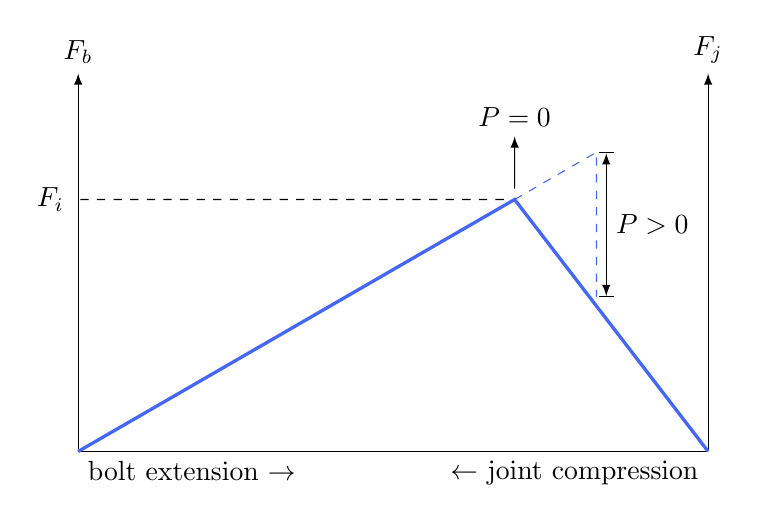
\begin{tikzpicture}[scale=0.8, >=latex]
    \draw [->] (0,0) node(A){} node[below right]{bolt extension $\rightarrow$} --++ (90:6) node[above]{$F_b$};
    \draw (0,0) --++ (0:10);
    \draw [->, xshift=10cm] (0,0) node(B){} node[below left]{$\leftarrow$ joint compression} --++ (90:6) node[above]{$F_j$};
    \draw [SkyBlue!50!Blue, very thick](A.center) --++ (30:8) node(C){} -- (B.center);
    \draw [SkyBlue!50!Blue, dashed] (C.center) --++ (30:1.5) node(D){} --++ (-90:2.3) node(E){};
     \draw [|<->|] (D.east) -- (E.east) node[midway, right]{$P>0$};
    \draw [dashed] (C) -- ++ (180:7) node[left]{$F_i$};
    \draw [->] (C) --++ (90:1) node[above]{$P=0$} ;
  \end{tikzpicture}
\end{figure} 
\end{frame}

\begin{frame}[label={sec:org939d4c3}]{Load Distribution in Tension Joints with External Tensile Load}
From previous diagram

\begin{align*} 
  {F_b} &= {P_b} + {F_i} = CP + {F_i} \\[1em]
  {F_j} &= (1 - C)P - {F_i}
\end{align*}

where \(C = k_b/(k_b + k_j)\).

Load carried by bolt and clamped members depend on stiffness ratio
\end{frame}

\begin{frame}[label={sec:org3dcb705}]{Bolted Joint Stiffness}
\begin{columns}
  \column{0.6\textwidth}
  \centering
  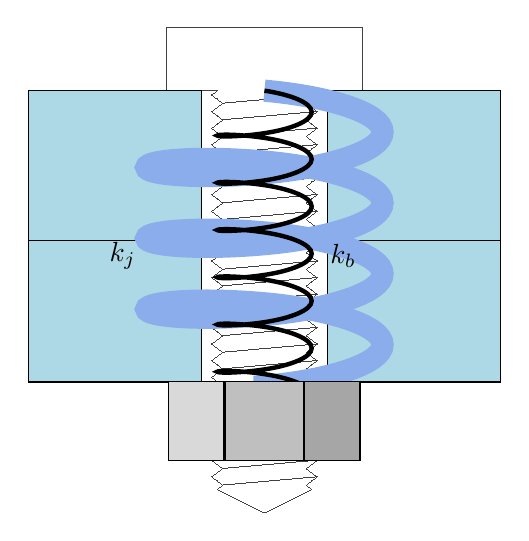
\begin{tikzpicture}[scale=1]
    \draw[decorate,line width=0pt,Black!50!Grey,decoration={screw, screw radius=0.6cm, thread amplitude=2pt, thread separation=3pt, head width=2.5cm, head length=0.8cm}] (0,5) -- (0,-1);
    % clamped members
    \draw[fill=LightBlue] (-3,0.5) rectangle (-0.8,2.3);
    \draw[fill=LightBlue, xshift=3.8cm] (-3,0.5) rectangle (-0.8,2.3);
    \draw[fill=LightBlue] (-3,2.3) rectangle (-0.8,4.2);
    \draw[fill=LightBlue, xshift=3.8cm] (-3,2.3) rectangle (-0.8,4.2);
  % springs
    \draw[decoration={aspect=0.2, segment length=9mm, amplitude=1.5cm,coil},decorate, line width=8pt, LightBlue!80!Blue] (0,4.2) -- (0,0) node(A){} node[midway, black, xshift=-1.8cm]{$k_j$};
    \draw[decoration={aspect=0.2, segment length=6mm, amplitude=0.6cm,coil},decorate, ultra thick] (0,4.2) --  (0,0) node[midway,black, xshift=1cm]{$k_b$};
    % nut
    \node at (0,-0.5) [anchor=south, draw, rectangle, fill=Grey!50, minimum height=1cm, minimum width=1cm](B){};
    \node at (B.east) [anchor=west, draw, rectangle, fill=Grey!70, minimum height=1cm, minimum width=0.7cm]{};
    \node at (B.west) [anchor=east, draw, rectangle, fill=Grey!30, minimum height=1cm, minimum width=0.7cm]{};
  \end{tikzpicture}
  \column{0.4\textwidth}
  \normalcolor
  \Large{ $k_{total} = k_b + k_j$ }
\end{columns}
\end{frame}

\begin{frame}[label={sec:org8c206a0}]{Bolt Size Selection for Tension Joints}
The only job we have is to keep the clamped part together
\begin{gather*}
  F_j = 0 = (1 - C)P - {F_i} \\ 
  P = \frac{F_i}{1 - C}
\end{gather*}

For non-permanent joints, \(F_i = 0.75 S_p A_t\) and \(C \approx 0.25\)

For the bolted joint to have a safety factor of \(N_s\)

\begin{equation*}
  {A_t} = \frac{N_sP}{N S_p}
\end{equation*}
\end{frame}

\begin{frame}[label={sec:org89bf6f4}]{Friction Joints}
\begin{columns}
  \column{0.7\textwidth}
  \centering
  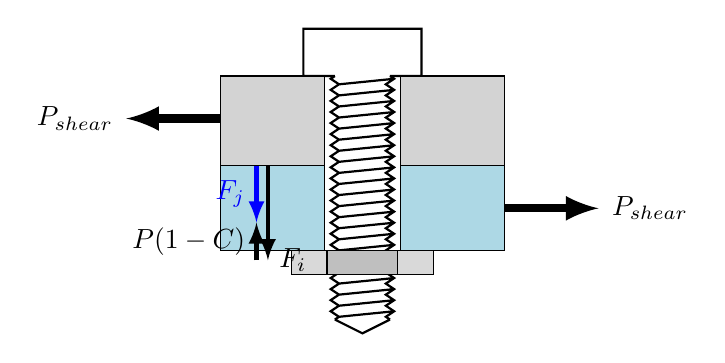
\begin{tikzpicture}[>=latex, scale=0.6]
    \draw[decorate,thick,decoration={screw, screw radius=0.35cm, thread amplitude=1.5pt, thread separation=2pt, head width=1.5cm, head length=0.6cm}] (0,5.2) -- (0,-1);
    % clamped members
    \draw[fill=LightBlue] (-3,0.5) rectangle (-0.8,2.3);
    \draw[fill=LightBlue, xshift=3.8cm] (-3,0.5) rectangle (-0.8,2.3);
    \draw[fill=LightGrey] (-3,2.3) rectangle (-0.8,4.2);
    \draw[fill=LightGrey, xshift=3.8cm] (-3,2.3) rectangle (-0.8,4.2);
    % nut
    \draw[fill=Grey!30] (-1.5,0) rectangle (-0.75,0.5);
    \draw[fill=Grey!30] (0.75,0) rectangle (1.5,0.5);
    \draw[fill=Grey!50] (-0.75,0) rectangle (0.75,0.5);
    % forces
    \draw[->, ultra thick] (-2,2.3) --++ (-90:2) node (A){} node[right]{$F_i$};
    \draw[->, ultra thick] (A.west) --++ (90:0.8) node (B){} node[midway,left]{$P(1-C)$};
    \draw[<-, ultra thick, Blue]  (B.center) --++ (90:1.2) node[midway,left]{$F_j$};
    \draw[->, line width=3pt] (-3,3.3) --++ (180:2) node[left]{$P_{shear}$};
    \draw[->, line width=3pt] (3,1.4) --++ (0:2) node[right]{$P_{shear}$};
  \end{tikzpicture}
  \column{0.4\textwidth}
  \begin{itemize}
  \item Prevent members from sliding by \emph{friction} not interference
  \item Compressive load exerted by bolt generate friction
  \end{itemize}
\end{columns}
\end{frame}

\begin{frame}[label={sec:org6840dbd}]{Bolt Size Selection for Friction Joints}
\[{P_{shear}} = -\mu {F_j}\] 

Again assuming \$ F\textsubscript{i} = 0.75 S\textsubscript{p} A\textsubscript{t}\$ and \(C = 0.25\)

\begin{align*}
  P_{shear} &= -\mu {F_j} = -\mu \left( P(1 - C) - F_i \right) \\
            &= \mu (0.75{S_p}{A_t} - 0.75P) \\
  A_t &= \frac{1}{S_p}\left( \frac{P_{shear}}{0.75 \mu} + P \right)
\end{align*}

For safety factor \(N_s\) with \(N\) bolts

\begin{gather*}
  A_t = \frac{N_s}{N S_p}\left( \frac{P_{shear}}{0.75 \mu} + P \right)
\end{gather*}
\end{frame}


\begin{frame}[label={sec:orgfbc900e}]{Flange Joints}
\begin{itemize}
\item Circular bolt arrays for sealing purpose.
\item Mainly used for pipe connections and pressure vessels
\end{itemize}
\begin{figure}[h]
  \centering
  \includegraphics[height=0.45\textheight]{pictures/pipe-connection}
  \includegraphics[height=0.45\textheight]{pictures/pressure-vessel}
\end{figure}
\end{frame}

\begin{frame}[label={sec:orgc3dcc31}]{Gasketed Flange Joints}
\begin{figure}[h]
  \includegraphics[height=0.4\textheight]{pictures/gasket-joint}
\end{figure}
\begin{itemize}
\item soft materials: rubber, plastic, or soft metals between clamped member
\item How does that help?
\item How does it effect the joint strength?
\end{itemize}
\end{frame}

\begin{frame}[label={sec:orgb314297}]{Equation for Flange Joints}
\centering
\begin{tikzpicture}[>=latex]
  \node {\includegraphics[width=0.8\textwidth]{pictures/flange-joint}};
  \draw [|<->|, thick] (0.6,1.35) --++ (-90:2.9) node[midway, left]{$D_b$};
\end{tikzpicture}
$$ 3 \leqslant \frac{\pi D_b}{Nd} \leqslant 6 $$
\end{frame}

\begin{frame}[label={sec:orgef2dbb8}]{Flange Joint on Pressure Vessel Example}
A cylindrical pressure vessel is pressurized to 10 MPa. The cross section of the vessel is shown below. The flange joint to keep the cover on the vessel is made up of 12 grade 12.9 M8 coarse thread bolts. Is this joint safe? If not, determine the proper bolt size.
\begin{figure}[h]
  \centering
  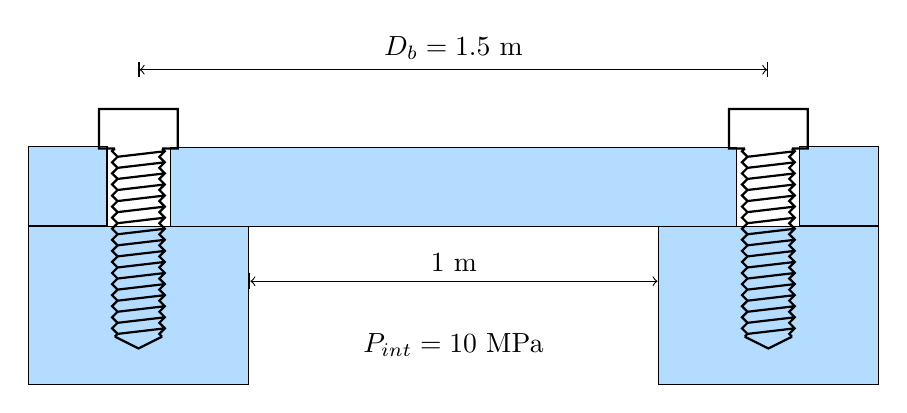
\begin{tikzpicture}
    % clamped members left
    \node at (0,-0.5) [anchor=south,draw, rectangle, fill=lightblue, minimum width=2.8cm, minimum height=2cm](A){};
    \node at (A.north west) [anchor=south west,draw, rectangle, fill=lightblue, minimum width=1cm, minimum height=1cm]{};
  % clamped members right
    \node at (0,-0.5) [anchor=south,draw, rectangle, fill=lightblue, minimum width=2.8cm, minimum height=2cm, xshift=8cm](B){};
    \node at (B.north east) [anchor=south east,draw, rectangle, fill=lightblue, minimum width=1cm, minimum height=1cm]{};
    % cover
    \draw [fill=lightblue] (A.north east) ++ (-1,1) --++ (-90:1) -- (B.north west) --++ (1,0) --++ (90:1) --cycle;
    % bolt left
    \draw[decorate,thick,decoration={screw, screw radius=0.3cm, thread amplitude=1pt, thread separation=2pt, head width=1.0cm, head length=0.5cm}] (0,3) -- (0,0);
    % bolt right
    \draw[decorate,thick,decoration={screw, screw radius=0.3cm, thread amplitude=1pt, thread separation=2pt, head width=1.0cm, head length=0.5cm}, xshift=8cm] (0,3) -- (0,0);
    % internal pressure
    \node at (A.center) [xshift=4cm, yshift=-0.5cm]{$P_{int} = 10$ MPa};
    % dimensions
    \draw [|<->|] (0,3.5) --++ (0:8) node[midway, above]{$D_b = 1.5$ m};
    \draw [|<->|] (A.north east) ++ (-90:0.7) --++ (0:5.2) node[midway, above]{1 m};
  \end{tikzpicture}
\end{figure}
\end{frame}

\begin{frame}[label={sec:orgc94c492}]{Solution}
\begin{itemize}
  \item Assume constant pressure, $N_{s}$ = 2
        \[{A_t} = \frac{{P{N_s}}}{{{S_p}}}\]
  \item The vertical load comes from the pressure force, which is
        \[{P_{total}} = p\pi {r^2} = 10 \times {10^6} \times \pi  \times {0.5^2} = 7.85\;{\text{MN}}\]
\end{itemize}
\end{frame}

\begin{frame}[label={sec:orgf865377}]{Solutions}
\begin{itemize}
  \item We will assume that the load is distributed evenly on all 12 bolts, so that
        \[P = \frac{{{P_{total}}}}{N} = \frac{7.85 \text{ MN}}{12} = 6.54 \times {10^5}\;{\text{N}}\]
  \item Assume that we use the bolt material grade 12.9 whose proof strength is 970 MPa, the required tensile area is
        \[{A_t} = \frac{(2)(6.54 \times 10^5)}{970 \times 10^6} = 1.35 \times 10^{ - 3} \text{ m}^2 = 1350 \text{ mm}^{2}\]
\end{itemize}
\end{frame}

\begin{frame}[label={sec:org9336530}]{Solutions}
\begin{itemize}
  \item The calculated required tensile area, even with the strongest material (grade 12.9), is larger than M8 coarse thread (36.6 mm$^2$) and therefore the given design is unsafe!
  \item Redesigning the flange joint, it must satisfy the sizing equation above and the bolt distance equation, namely
        \[3 \leqslant \frac{\pi D_b}{Nd} \leqslant 6\]
  \item Since $D_{b}$ = 150 cm, set the inequality to 4.5 to solve.
      \begin{gather*}
        \frac{{\pi {D_b}}}{{Nd}} = 4.5 \hfill \\
        Nd = 1.05 \hfill \\
      \end{gather*}
\end{itemize}
\end{frame}

\begin{frame}[label={sec:org29893f4}]{Solutions}
\begin{itemize}
  \item Reapply the tension joint equation to determine the total required tensile area, we have
        \begin{align*}
          N{A_t} &= \frac{{{N_s}P}}{{{S_p}}} = \frac{2(7.85 \times 10^6)}{970 \times 10^6} \\
                 &= 1.62 \times 10^{ - 2} \text{ m}^2
        \end{align*}
\end{itemize}
\end{frame}

\begin{frame}[label={sec:org733d4e7}]{Solutions}
\begin{itemize}
  \item 2 equations, 3 unknowns
  \item Are the unknowns all independent?
  \end{itemize}
\[\begin{gathered}
    A_t \approx \frac{\pi}{4}\left(0.9d\right)^{2} \\
  NA_t \approx N(0.81)\frac{\pi}{4}{d^2} = 1.62 \times {10^{ - 2}} \\
  Nd^2 = 2.58 \times 10^{ - 2} \\
\end{gathered} \]
\end{frame}

\begin{frame}[label={sec:orge95eebf}]{Solutions}
\begin{itemize}
  \item Solving the system of equations, we have
\end{itemize}
\[\frac{Nd^2}{Nd} = \frac{2.58 \times 10^{-2}}{1.05} = 0.0245 \text{ m} = 24.5 \text{ mm} \]
\end{frame}

\begin{frame}[label={sec:org6852b98}]{Solutions}
\begin{itemize}
  \item Since there is no standard bolts with that size, we pick the next larger bolt, M27 $\times$ 2 (fine thread)
  \item Finally, $A_t$ = 496 mm$^2$ (from M27) is used to solve for the number of required bolts
        \[N = \frac{{1.62 \times {{10}^{ - 2}}}}{{496 \times {{10}^{ - 6}}}} = 25.4\]
  \item Therefore, we need 26 M27 $\times$ 2 for this flange joint.
\end{itemize}
\end{frame}

\section{Bolted Joint for Fatigue Loading}
\label{sec:org35eddb0}

\begin{frame}[label={sec:org3925696}]{Bolt Sizing for Fatigue Loading}
\begin{itemize}
\item If properly tightened, endurance limit of bolt is constant regardless of average stress
   $$ N_s = \frac{S_e}{\sigma_a} $$
   $$ \sigma_a = \frac{C K_f (P_{\max} - P_{\min})}{2NA_t} $$
\end{itemize}
\end{frame}

\begin{frame}[label={sec:orgd639498}]{Bolt Strength under Fatigue}
\centering
\begin{tabular}{lc}
  \toprule
  Material Grade & Endurance Limit ($S_e$) \\
  \midrule
  8.8 & 129 MPa \\
  9.8 & 140 MPa \\
  10.9 & 162 MPa \\
  12.9 & 190 MPa \\
  \bottomrule
\end{tabular}
\end{frame}

\begin{frame}[label={sec:org1065d89}]{Stress Concentration Factor of Bolts}
\begin{tabular}{>{\raggedright}p{2.5cm}>{\raggedright}p{2.5cm}>{\raggedright}p{2cm}>{\raggedright\arraybackslash}p{2cm}}
  \toprule
  Hardness & SAE Class (ISO Threads) & $K_f$ Rolled threads & $K_f$ Cut threads \\
  \midrule
  Below 200 Bhn (annealed) & 5.8 and below & 2.2 & 2.8 \\
  Above 200 Bhn (hardened) & 8.8 and above & 3.0 & 3.8 \\
  \bottomrule
\end{tabular}
\end{frame}

\begin{frame}[label={sec:org73140a1}]{Bolted Joint Design under Fatigue Example}
A cylindrical pressure vessel is pressurized and depressurized repeatedly between 0 and 10 MPa during its operation. The cross section of the vessel is shown below. Design a proper flange joint with a safety factor of 2.

\begin{figure}[h]
  \centering
  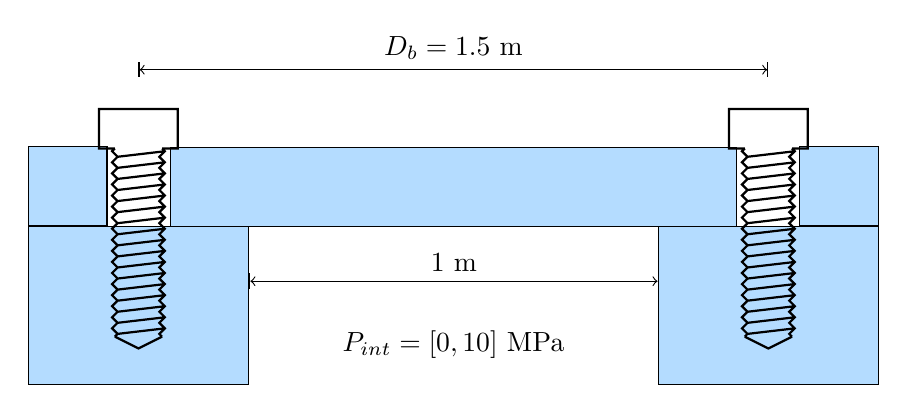
\begin{tikzpicture}
    % clamped members left
    \node at (0,-0.5) [anchor=south,draw, rectangle, fill=lightblue, minimum width=2.8cm, minimum height=2cm](A){};
    \node at (A.north west) [anchor=south west,draw, rectangle, fill=lightblue, minimum width=1cm, minimum height=1cm]{};
  % clamped members right
    \node at (0,-0.5) [anchor=south,draw, rectangle, fill=lightblue, minimum width=2.8cm, minimum height=2cm, xshift=8cm](B){};
    \node at (B.north east) [anchor=south east,draw, rectangle, fill=lightblue, minimum width=1cm, minimum height=1cm]{};
    % cover
    \draw [fill=lightblue] (A.north east) ++ (-1,1) --++ (-90:1) -- (B.north west) --++ (1,0) --++ (90:1) --cycle;
    % bolt left
    \draw[decorate,thick,decoration={screw, screw radius=0.3cm, thread amplitude=1pt, thread separation=2pt, head width=1.0cm, head length=0.5cm}] (0,3) -- (0,0);
    % bolt right
    \draw[decorate,thick,decoration={screw, screw radius=0.3cm, thread amplitude=1pt, thread separation=2pt, head width=1.0cm, head length=0.5cm}, xshift=8cm] (0,3) -- (0,0);
    % internal pressure
    \node at (A.center) [xshift=4cm, yshift=-0.5cm]{$P_{int} = [0,10]$ MPa};
    % dimensions
    \draw [|<->|] (0,3.5) --++ (0:8) node[midway, above]{$D_b = 1.5$ m};
    \draw [|<->|] (A.north east) ++ (-90:0.7) --++ (0:5.2) node[midway, above]{1 m};
  \end{tikzpicture}
\end{figure}
\end{frame}


\begin{frame}[label={sec:orge5fc244}]{Solution}
\begin{itemize}
\item Definitely fatigue related
\item Max load = 7.85 MN, from previous example
\item Min load = ?
\end{itemize}

\begin{align*}
  \sigma_{\max} &= \frac{C K_f P_{\max}}{N A_t} = \frac{0.25(3)(7.85 \times 10^6)}{NA_t} = \frac{5.89 \times 10^6}{NA_t} \\
  \sigma _{\min} &= 0 \\
  \sigma _a &= \frac{2.94 \times 10^6}{N A_t}
\end{align*}
\end{frame}

\begin{frame}[label={sec:org5a96309}]{Solutions}
\begin{itemize}
\item Grade 12.9 $\rightarrow$ $S_e$ = 190 MPa
\end{itemize}

\[\begin{gathered}
   {N_s} = 2 = \frac{{{S_e}}}{{{\sigma _a}}} = \frac{{190 \times {{10}^6}}}{{\dfrac{{2.94 \times {{10}^6}}}{{N{A_t}}}}} \hfill \\
   N{A_t} = 3.10 \times 10^{ - 2} \text{ m}^2 \hfill \\
 \end{gathered} \]

\begin{itemize}
\item Check for yield under tensile load.
\end{itemize}

\[N{A_t} = \frac{{{N_s}P}}{{{S_p}}} = \frac{{2(7.85 \times {{10}^6})}}{{970 \times {{10}^6}}} = 1.62 \times {10^{ - 2}} \text{ m}^2\]
\end{frame}

\begin{frame}[label={sec:org0d2bc36}]{Solutions}
\begin{itemize}
  \item Fatigue requires larger area $\rightarrow$ deciding factor
\end{itemize}

\[\begin{gathered}
   \frac{{\pi {D_b}}}{{Nd}} = 4.5 \hfill \\
   Nd = 1.05 \hfill \\
 \end{gathered} \]

\begin{itemize}
  \item We can then solve for the required diameter.
\end{itemize}

\[\begin{gathered}
   N{A_t} = N(0.8)\frac{\pi}{4}{d^2} = 3.10 \times {10^{ - 2}} \hfill \\
   N{d^2} = 4.93 \times {10^{ - 2}} \hfill \\
   \frac{Nd^2}{Nd} = \frac{4.93 \times 10^{ - 2}}{1.05} = 0.047 \text{ m} \hfill \\
 \end{gathered} \]
\end{frame}

\begin{frame}[label={sec:org0e9cc78}]{Solutions}
\begin{itemize}
  \item The required bolts are then M48 $\times$ 5, and the required number of bolts is
        \[N = \frac{{3.10 \times {{10}^{ - 2}}}}{{1473 \times {{10}^{ - 6}}}} = 21\]
  \item So we would need 21 M48 $\times$ 5 bolts.
\end{itemize}
\end{frame}

\begin{frame}[label={sec:org2ea3706}]{Final Notes on Bolted Joint Design for Fatigue Loading}
\begin{itemize}
\item Properly tighten bolt
\item Choose rolled threads whenever possible
\end{itemize}
\end{frame}

\begin{frame}[label={sec:orgbfbcfac}]{Solutions}
\Huge \centering Any Questions?
\end{frame}
\end{document}